\providecommand{\main}{../../../..}
\documentclass[\main/dresen_thesis.tex]{subfiles}
\begin{document}
  \label{sec:looselyPackedNS:layers:sem}
  \begin{figure}[tb]
    \centering
    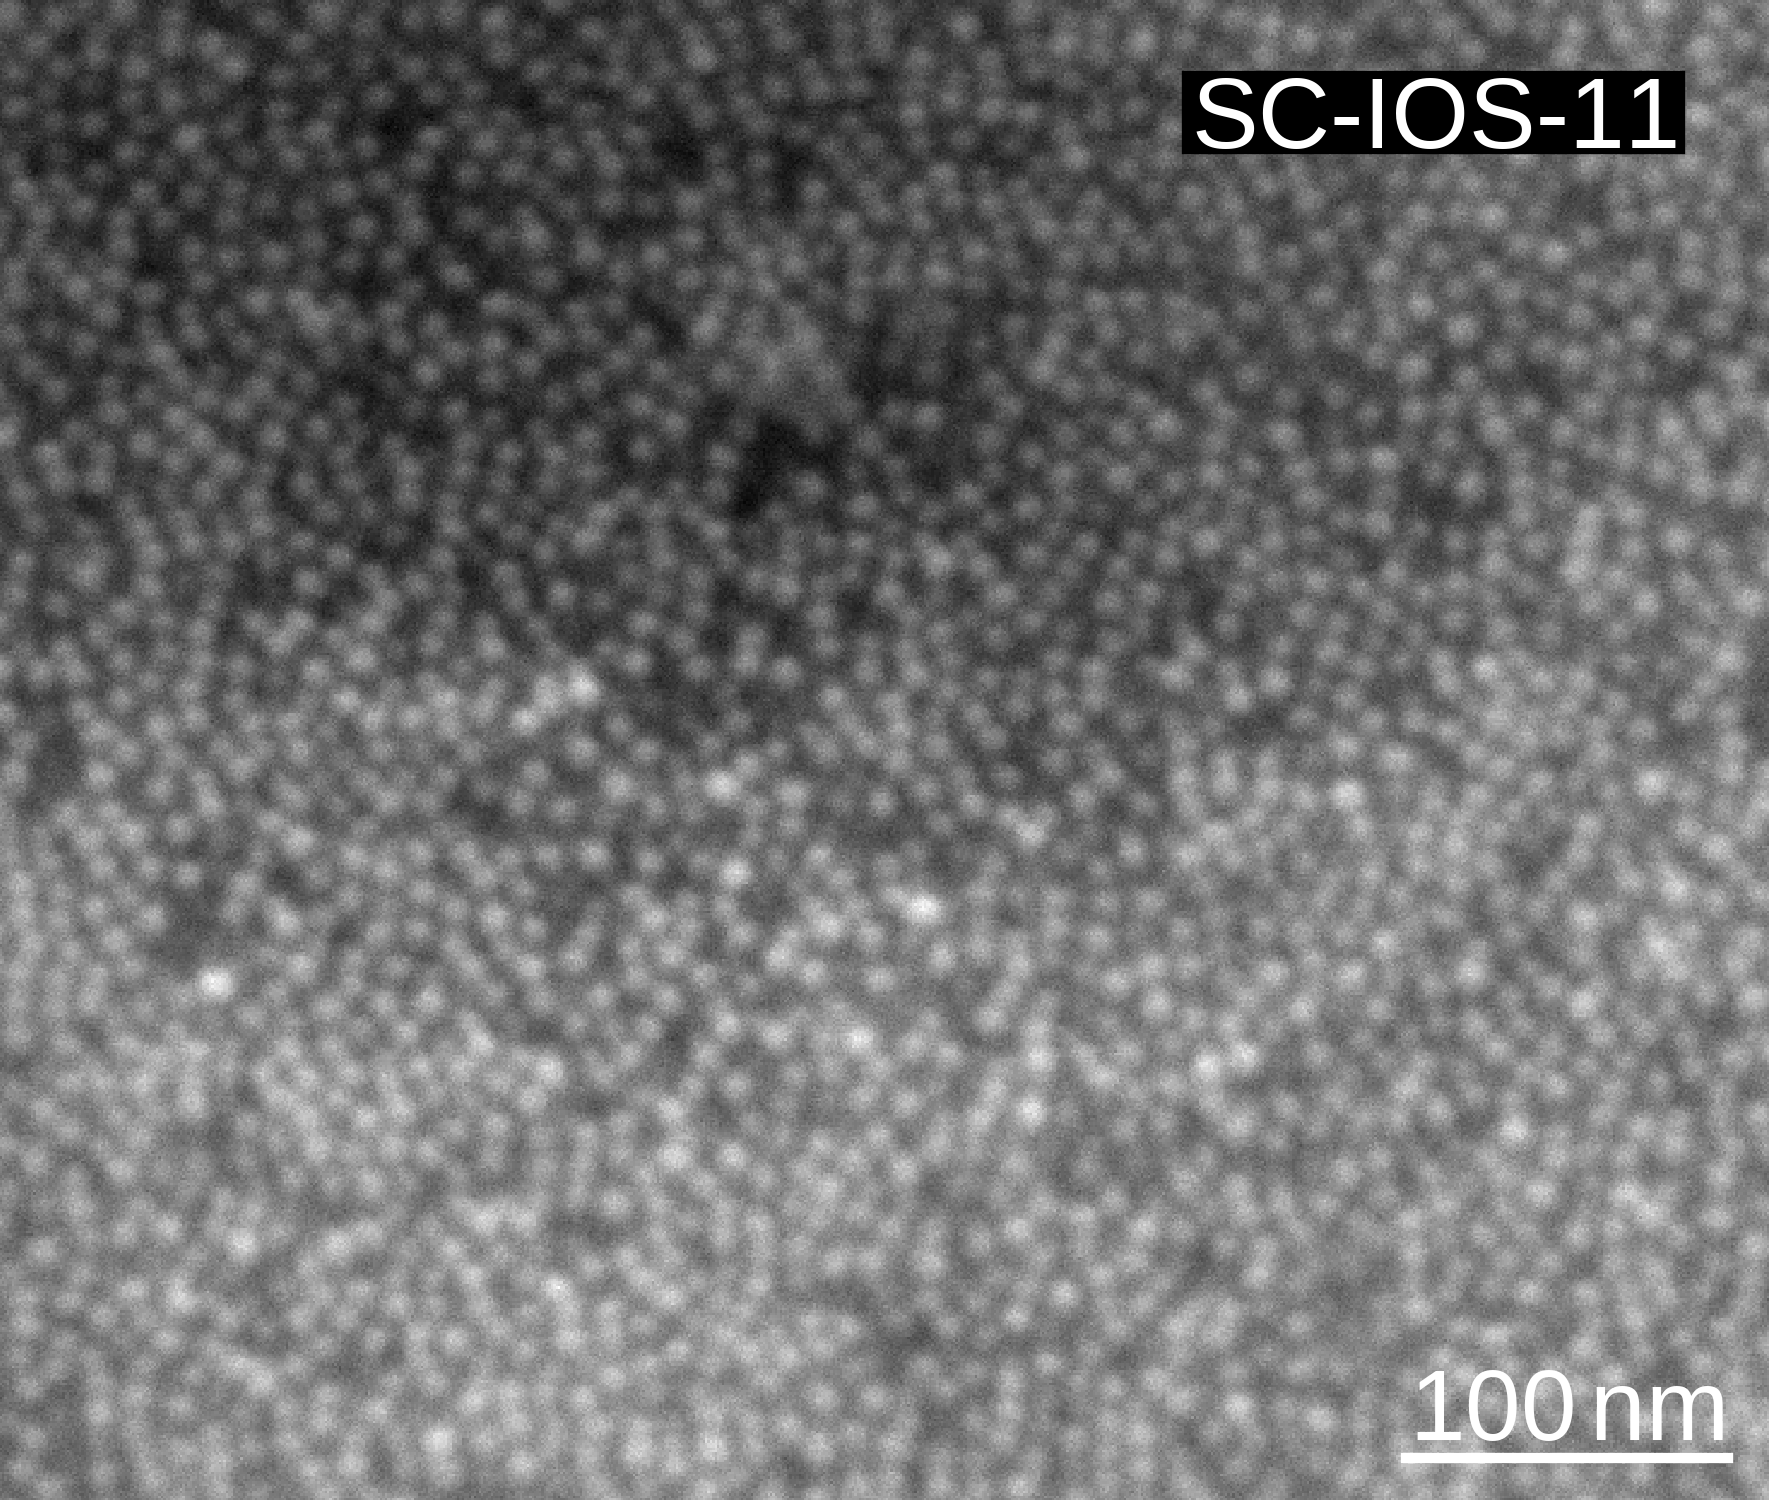
\includegraphics{looselyPackedNP_SEM_SC-IOS-11_TopView}
    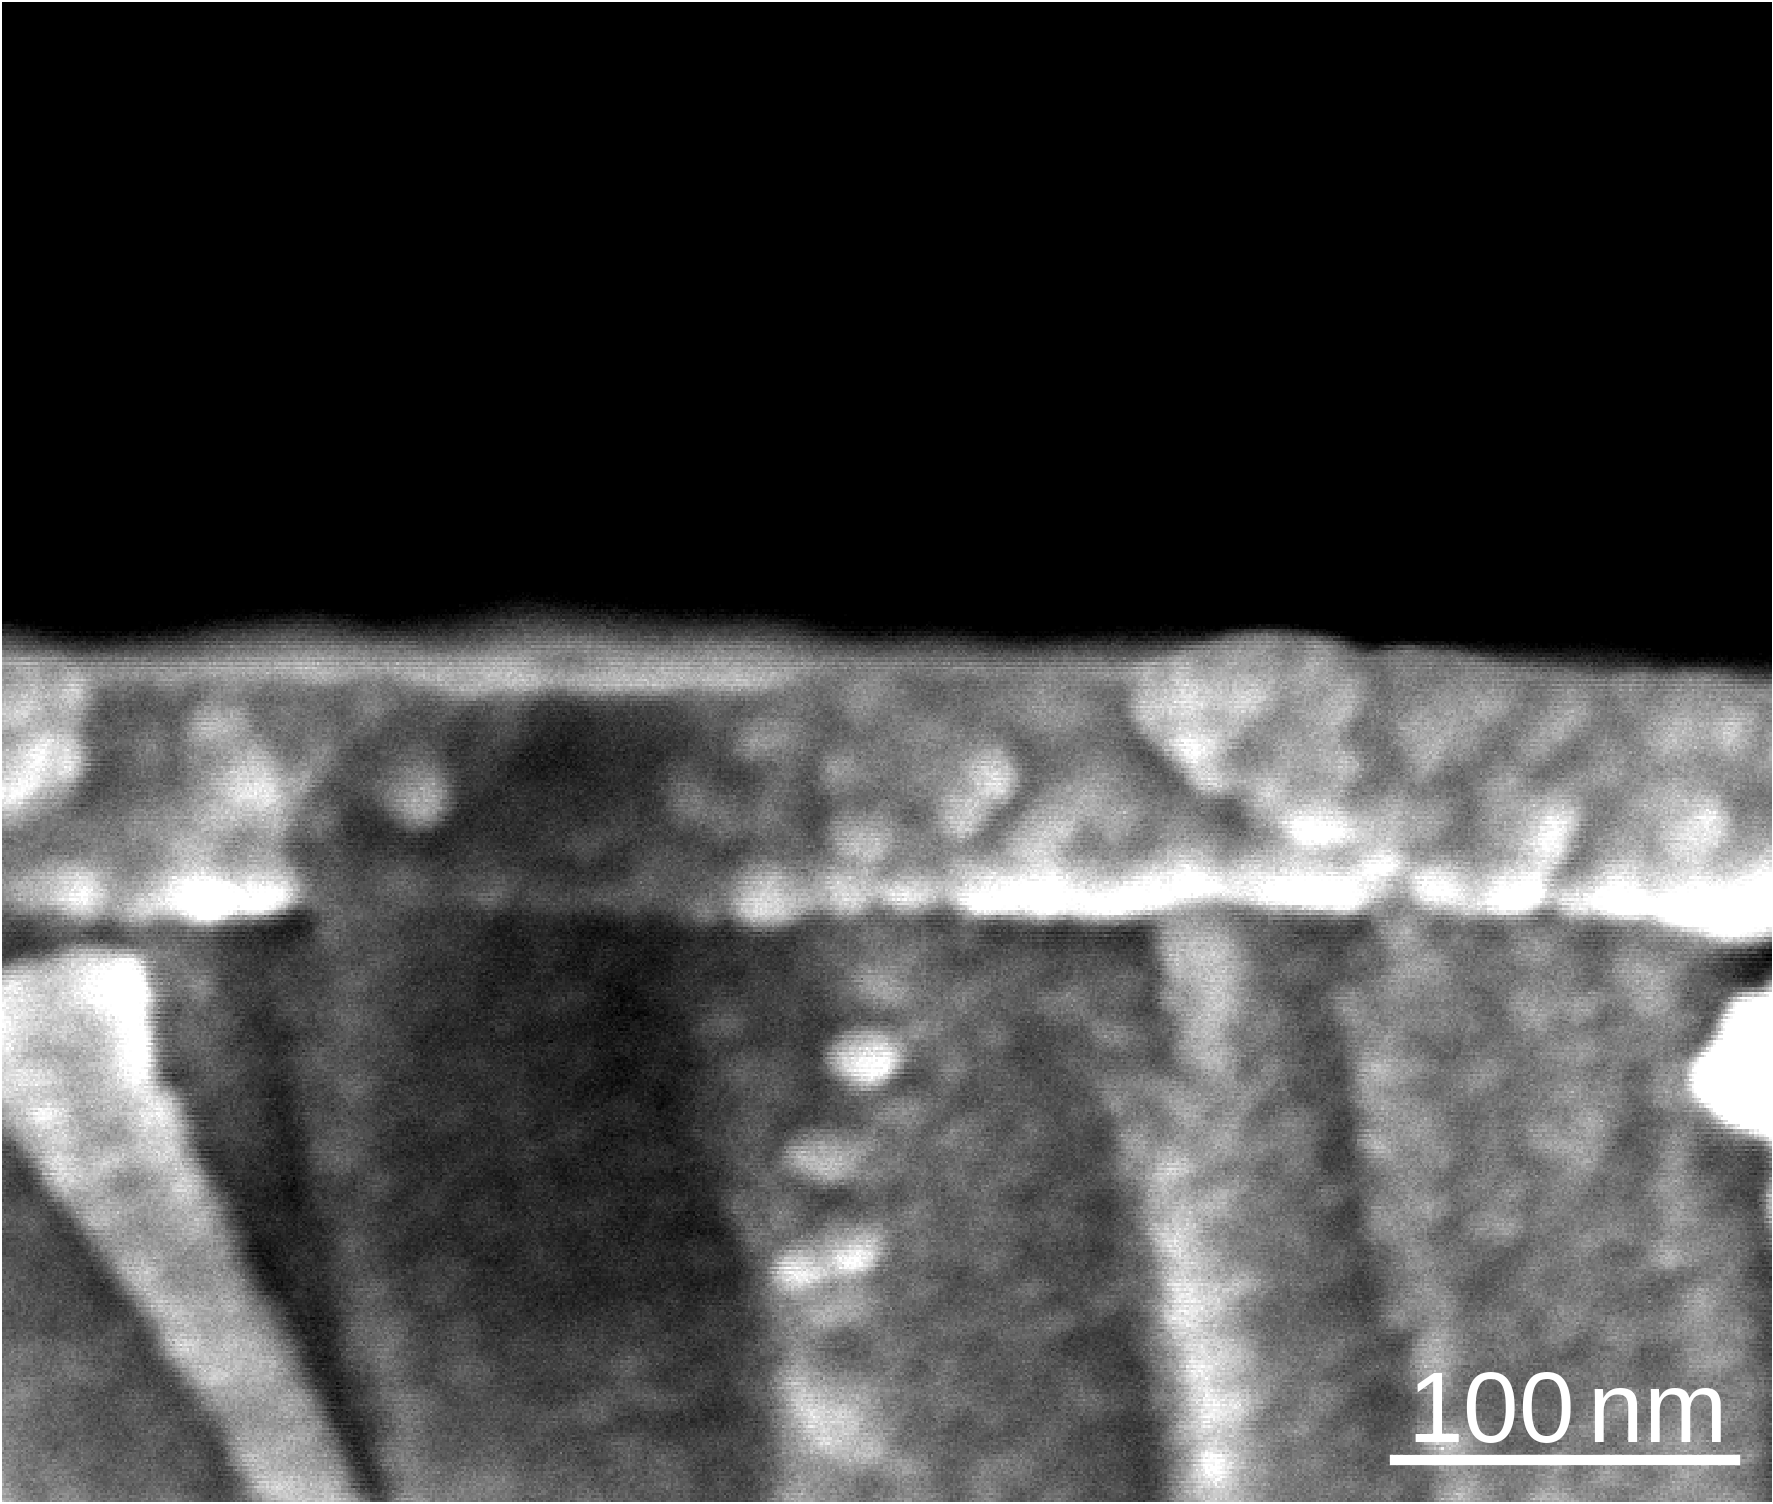
\includegraphics{looselyPackedNP_SEM_SC-IOS-11}
    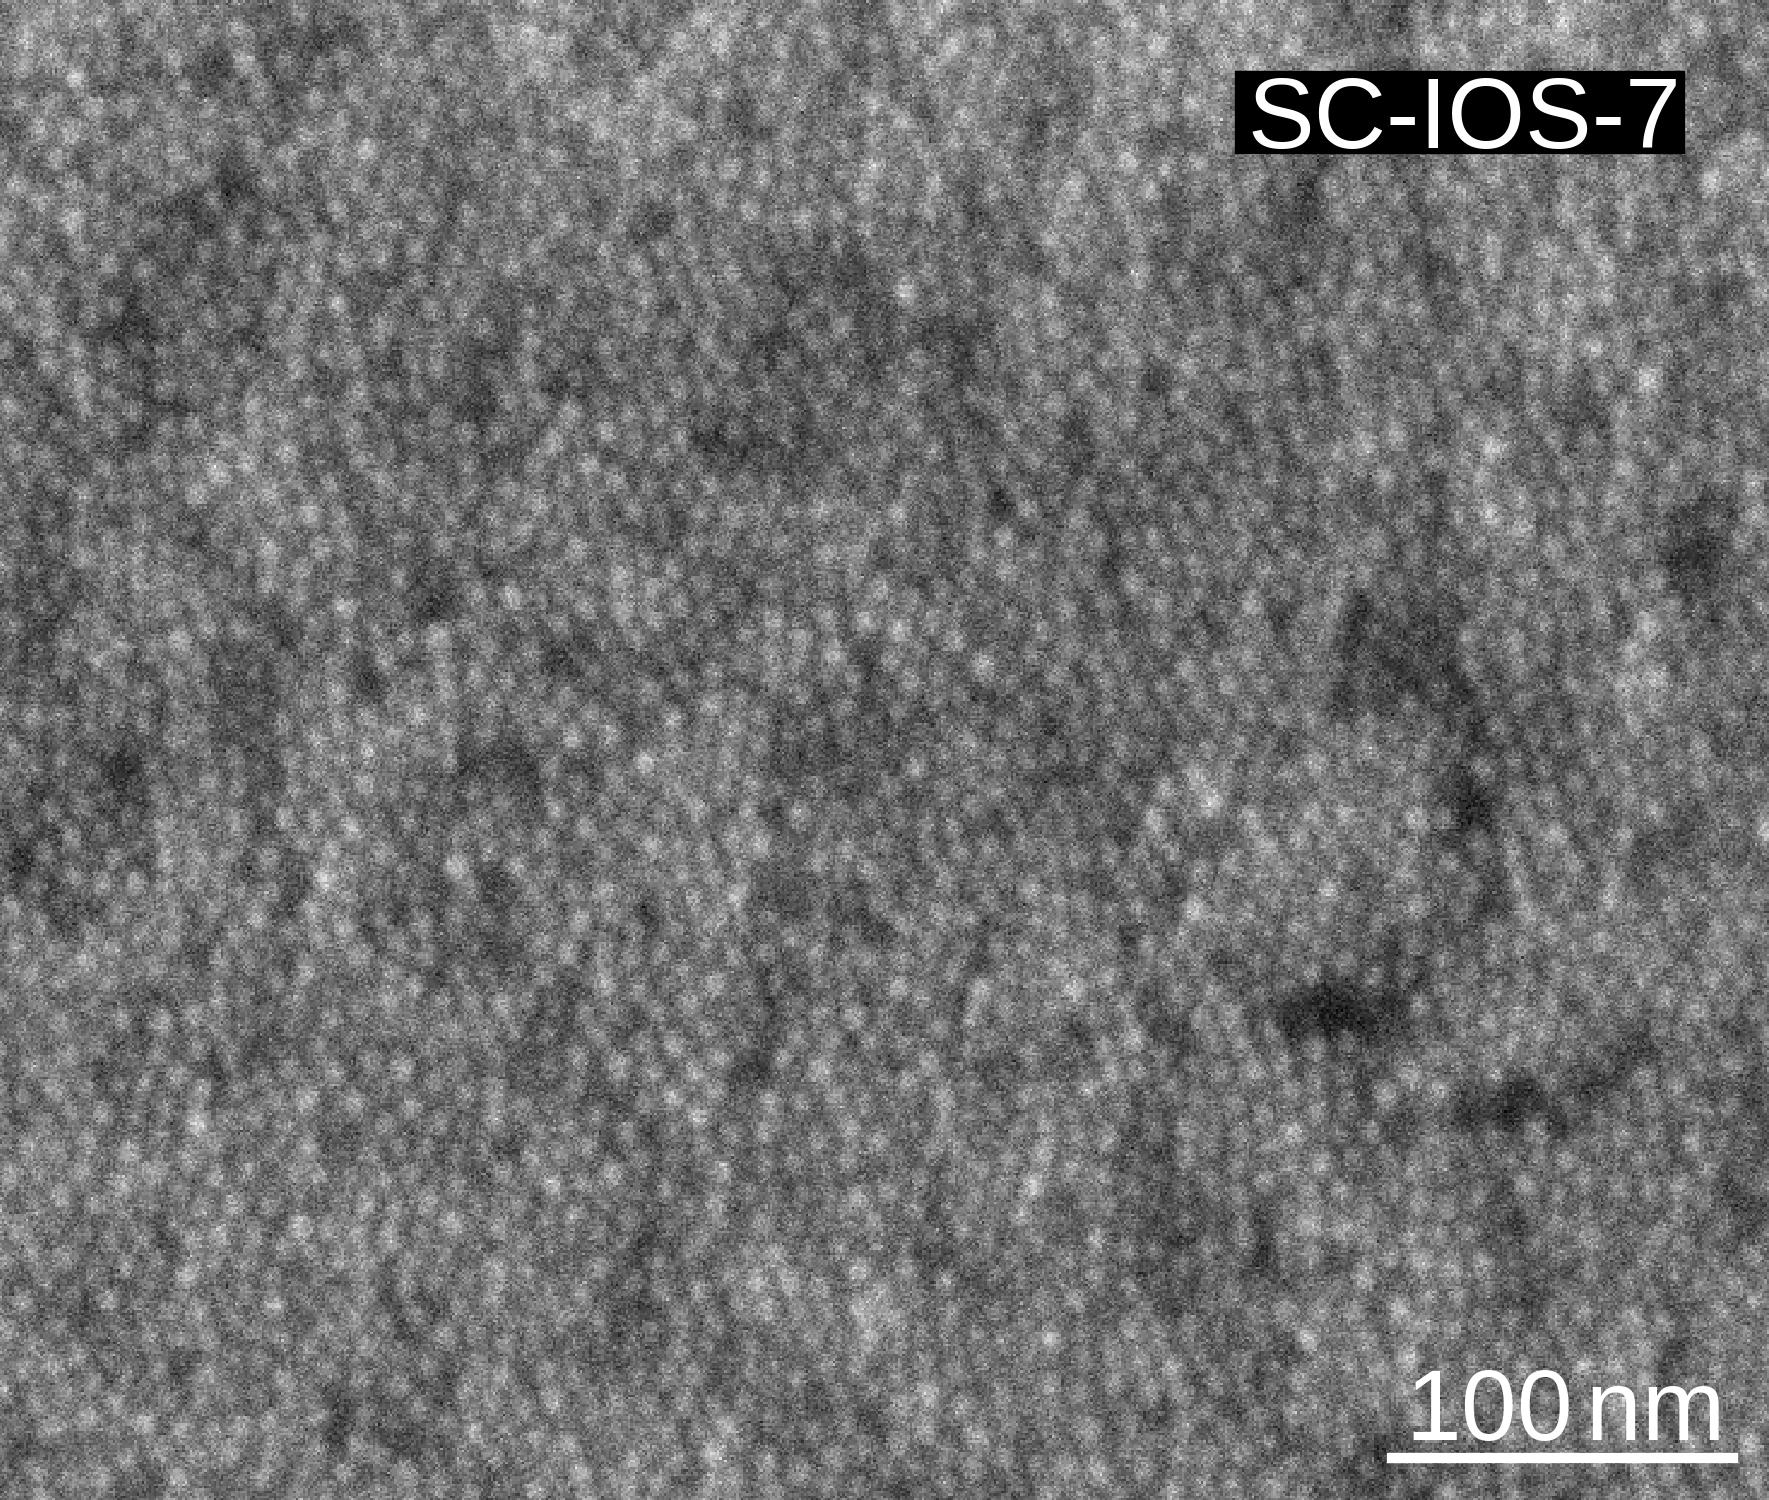
\includegraphics{looselyPackedNP_SEM_SC-IOS-7_TopView}
    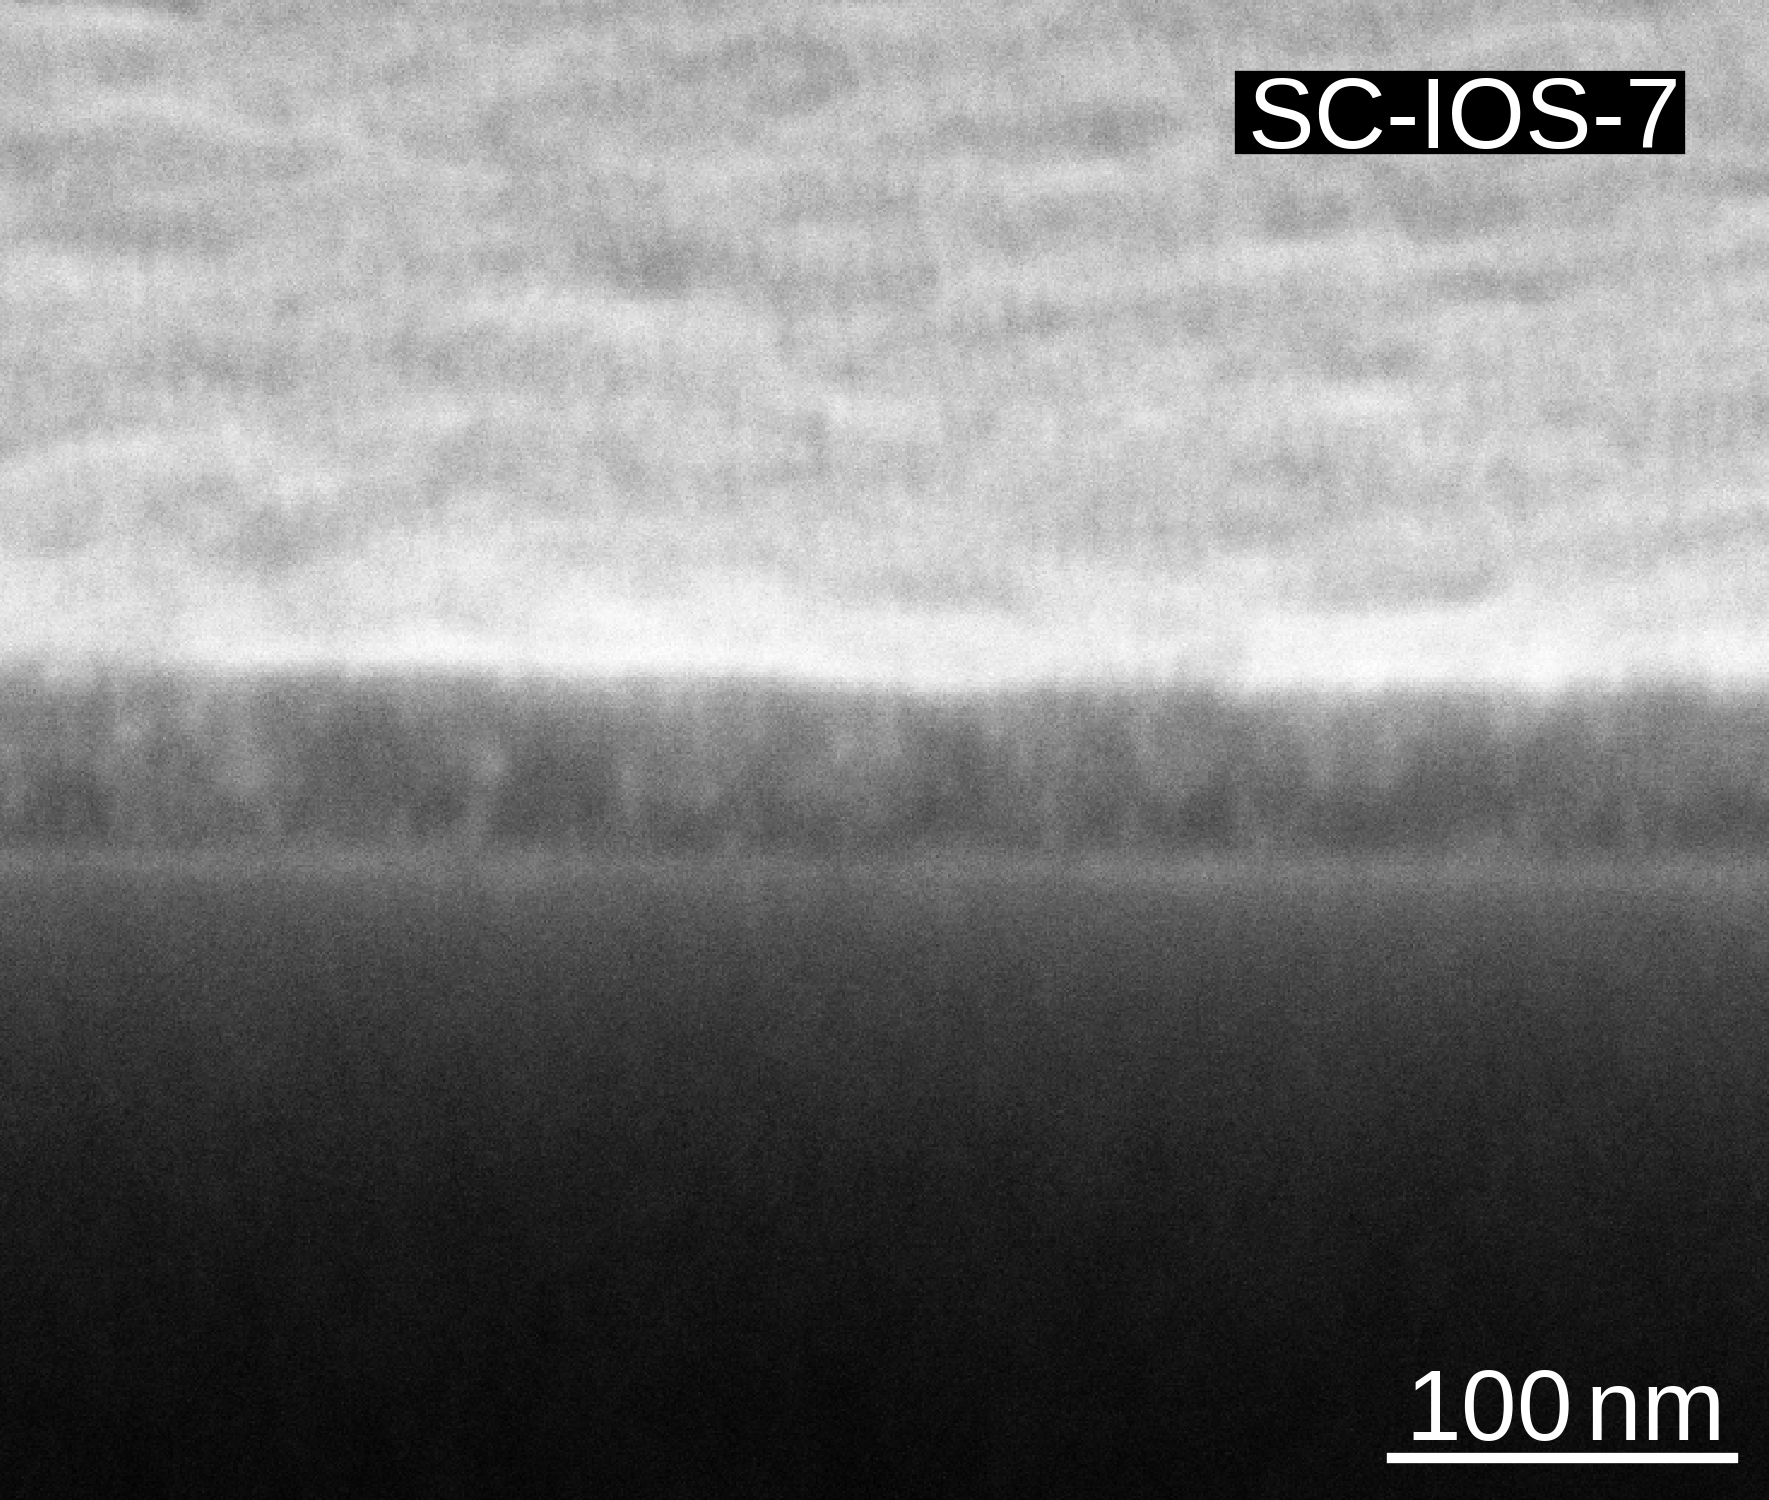
\includegraphics{looselyPackedNP_SEM_SC-IOS-7}
    \caption{\label{fig:looselyPackedNP:nuclearStructure:sem}SEM micrographs view of SC-IOS-11 viewed from the top (left) and in cross-section (right).}
  \end{figure}
  By using scanning electron microscopy, micrographs of the local structure are obtained for both SC-IOS-11  and SC-IOS-7 in \reffig{fig:looselyPackedNP:nuclearStructure:sem}.
  At close inspection of the top view, voids can be seen in both structures, which alludes to a loose packing of the spheres.
  Furthermore, the top view shows no long range order among the nanoparticles.

  The cross-sectional view shows in both cases a relative homogeneous layer of nanospheres with only a low surface roughness.
  The low surface roughness of the samples is expected for a spin-coated sample and is also a prerequisite to be able to study the sample quantitatively with reflectometry experiments in the following.
  The thickness of the layer is estimated from the cross-sectional images to $65 \unit{nm}$ for SC-IOS-11 and $55 \unit{nm}$ for SC-IOS-7.

  % Spheres that do not undergo any ordering process and are packed randomly have been studied extensively on the macroscopic scale \cite{Torquato_2000_IsRan} and it has been shown experimentally that the densest random close packing (RCP) lies in the order of $\approx 64 \, \%$.
  % In a long range ordered crystalline structure, the closest packing spheres can achieve are the face-centered cubic and the hexagonal close-packed structure, which have a packing of $74 \, \%$.
  % To study the packing of the nanoparticles, X-ray and neutron scattering provide non-destructive tools to quantify the order of the volume fraction across a large area of the sample.
  % X-ray and neutron reflectometry is used to study the vertical structure of the sample, and grazing incidence small-angle X-ray scattering to study the lateral structure.

  % \begin{figure}[tb]
  %   \centering
  %   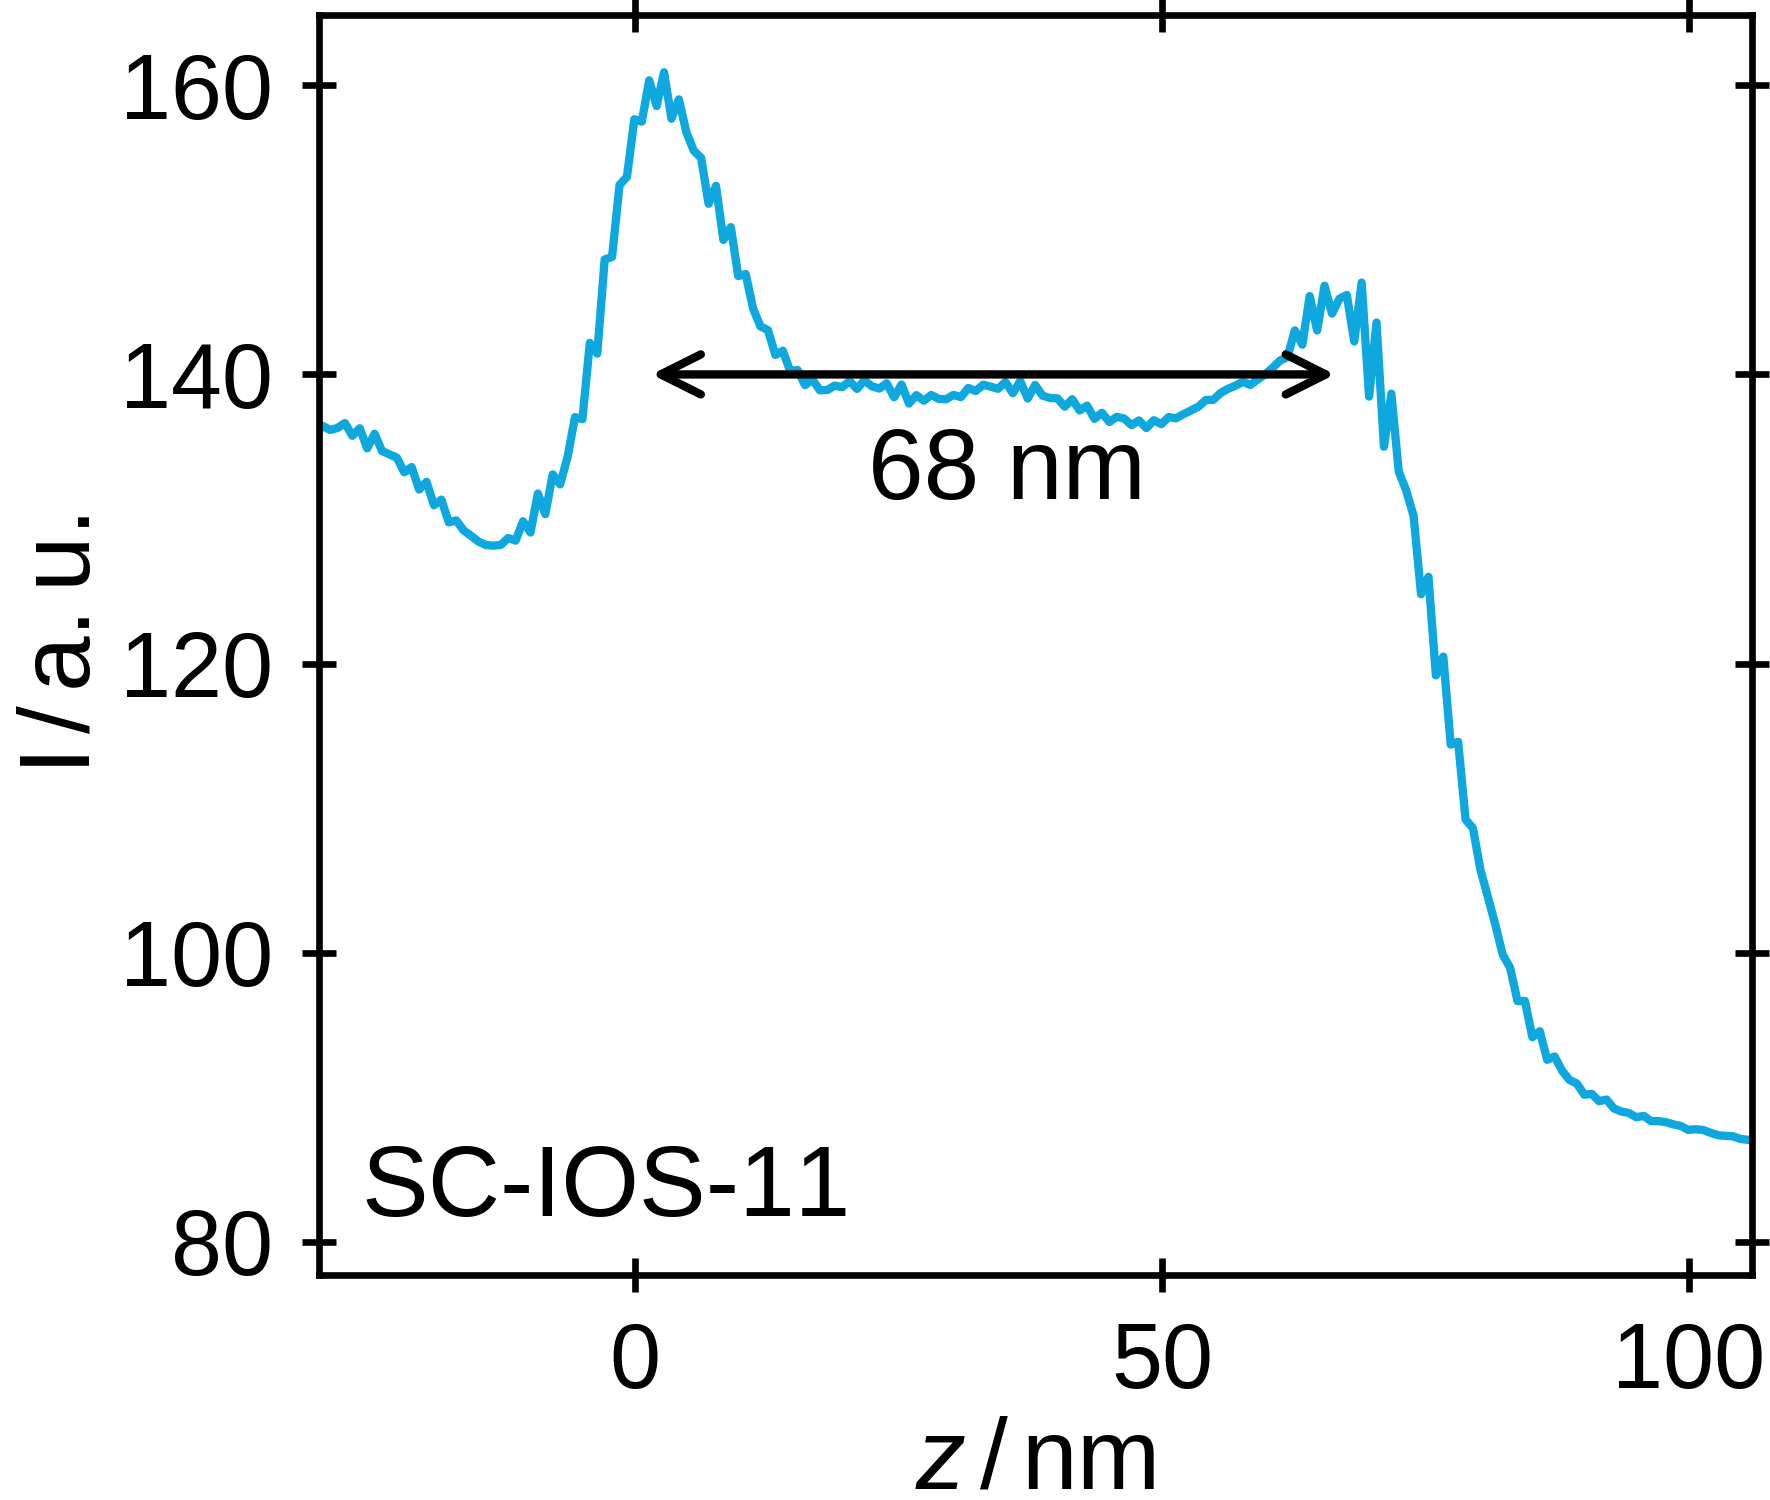
\includegraphics{looselyPackedNP_SEMprojection_SC-IOS-11}
  %   \caption{\label{fig:looselyPackedNP:nuclearStructure:semProjection}Projection of the pixel intensity along the vertical axis from the cross-sectional SEM shown in \reffig{fig:looselyPackedNP:nuclearStructure:sem}.}
  % \end{figure}
\end{document}